\chapter{Implementation and Block Diagrams}

The 4-bit ALU implementation consists of three main functional blocks: the Adder/Subtractor unit for arithmetic operations, the Multiplier unit, and the Logic Operations unit. Each block is designed with discrete digital components and controlled by selection signals.

\section{Adder/Subtractor Block Diagram}

The adder/subtractor circuit uses a 4-bit ripple-carry adder with XOR gates for two's complement subtraction. The control signal determines whether the operation is addition or subtraction.

\begin{figure}[h]
    \centering
    % ============================================
    % UNCOMMENT THE LINE BELOW AND ADD YOUR IMAGE
    % ============================================
    % \includegraphics[width=0.9\textwidth]{adder_subtractor}
    \fbox{\parbox{0.85\textwidth}{
        \vspace{6cm}
        \centering
        \textbf{[Insert Adder/Subtractor Block Diagram Here]}
        
        \textit{File name: adder\_subtractor.png}
        \vspace{0.5cm}
    }}
    \caption{4-Bit Adder/Subtractor Block Diagram showing the ripple-carry adder structure with XOR gates for two's complement generation}
    \label{fig:adder-subtractor}
\end{figure}

\textbf{Key Components:}
\begin{itemize}
    \item 4-bit Full Adder (74LS83 or discrete implementation using half adders)
    \item XOR gates for two's complement generation during subtraction
    \item Control signal (Add/Sub) for operation selection
    \item Carry output and overflow detection circuitry
    \item 4-bit input ports A and B
    \item 4-bit output port for Sum/Difference
\end{itemize}

\textbf{Operation:}
\begin{itemize}
    \item \textbf{Addition Mode:} When control signal is 0, the circuit performs A + B
    \item \textbf{Subtraction Mode:} When control signal is 1, the circuit performs A - B using two's complement (A + \textoverline{B} + 1)
\end{itemize}

\section{Multiplier Block Diagram}

The 4-bit multiplier uses the shift-and-add algorithm implemented with AND gates and adders to perform binary multiplication. The output is an 8-bit result to accommodate the full product range.

\begin{figure}[h]
    \centering
    % ============================================
    % UNCOMMENT THE LINE BELOW AND ADD YOUR IMAGE
    % ============================================
    % 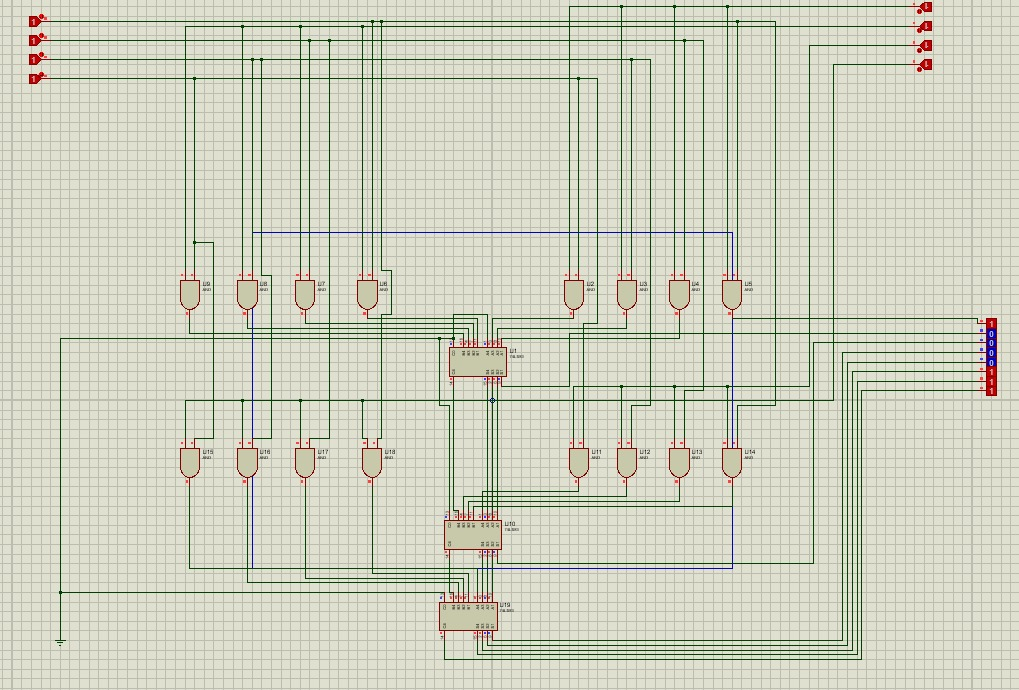
\includegraphics[width=0.9\textwidth]{multiplier}
    \fbox{\parbox{0.85\textwidth}{
        \vspace{6cm}
        \centering
        \textbf{[Insert Multiplier Block Diagram Here]}
        
        \textit{File name: multiplier.png}
        \vspace{0.5cm}
    }}
    \caption{4-Bit Multiplier Block Diagram using shift-and-add algorithm with AND gate arrays and multi-stage adders}
    \label{fig:multiplier}
\end{figure}

\textbf{Key Components:}
\begin{itemize}
    \item AND gate arrays (4×4 = 16 AND gates) for partial product generation
    \item Multi-stage full adders for partial product summation
    \item 8-bit output register for final product result
    \item Two 4-bit input ports (Multiplicand and Multiplier)
\end{itemize}

\textbf{Operation:}
\begin{itemize}
    \item Each bit of the multiplier is ANDed with all bits of multiplicand
    \item Partial products are shifted and added using full adder chains
    \item Final 8-bit product = Multiplicand × Multiplier
\end{itemize}

\section{Logic Operations Block Diagram}

The logic unit performs bitwise operations (AND, OR, XOR) on 4-bit inputs using basic logic gates with parallel implementation. A multiplexer selects the desired operation output.

\begin{figure}[h]
    \centering
    % ============================================
    % UNCOMMENT THE LINE BELOW AND ADD YOUR IMAGE
    % ============================================
    % \includegraphics[width=0.9\textwidth]{logic_operations}
    \fbox{\parbox{0.85\textwidth}{
        \vspace{6cm}
        \centering
        \textbf{[Insert Logic Operations Block Diagram Here]}
        
        \textit{File name: logic\_operations.png}
        \vspace{0.5cm}
    }}
    \caption{Logic Operations Block Diagram showing parallel implementation of bitwise AND, OR, and XOR operations with multiplexer-based output selection}
    \label{fig:logic-operations}
\end{figure}

\textbf{Key Components:}
\begin{itemize}
    \item 4 × AND gates (74LS08) for bitwise AND operation
    \item 4 × OR gates (74LS32) for bitwise OR operation
    \item 4 × XOR gates (74LS86) for bitwise XOR operation
    \item 4-bit 3-to-1 multiplexer for operation selection
    \item Two 4-bit input ports A and B
    \item 4-bit output port for result
\end{itemize}

\textbf{Operation:}
\begin{itemize}
    \item \textbf{AND Operation:} Each bit: $C_i = A_i \cdot B_i$ for $i = 0$ to $3$
    \item \textbf{OR Operation:} Each bit: $C_i = A_i + B_i$ for $i = 0$ to $3$
    \item \textbf{XOR Operation:} Each bit: $C_i = A_i \oplus B_i$ for $i = 0$ to $3$
\end{itemize}

\section{Complete ALU Integration}

The complete ALU integrates all functional blocks with a control unit that selects the desired operation based on control signals.

\begin{figure}[h]
    \centering
    % ============================================
    % UNCOMMENT THE LINE BELOW AND ADD YOUR IMAGE
    % ============================================
    % \includegraphics[width=\textwidth]{complete_alu}
    \fbox{\parbox{0.9\textwidth}{
        \vspace{7cm}
        \centering
        \textbf{[Insert Complete ALU Circuit Diagram Here]}
        
        \textit{File name: complete\_alu.png}
        \vspace{0.5cm}
    }}
    \caption{Complete 4-Bit ALU Circuit Diagram showing integration of all functional blocks with control unit}
    \label{fig:complete-alu}
\end{figure}

\textbf{Control Signal Mapping:}
\begin{table}
\captionabove{ALU Operation Control Signals}
\centering
\begin{tabular}{llll}
\toprule
\textbf{S2} & \textbf{S1} & \textbf{S0} & \textbf{Operation} \\
\midrule
0 & 0 & 0 & Addition \\
0 & 0 & 1 & Subtraction \\
0 & 1 & 0 & Multiplication \\
0 & 1 & 1 & Division \\
1 & 0 & 0 & AND \\
1 & 0 & 1 & OR \\
1 & 1 & 0 & XOR \\
1 & 1 & 1 & Reserved \\
\bottomrule
\end{tabular}
\label{tab:control-signals}
\end{table}
